\section{MATERIAL AND METHODS}
\begin{table}[H]
    \begin{tabular}{llcccc} \hline
    Station name   & Code       & Altitude (MSL) & Latitude   & Longitude    & Operating since \\ \hline
    Obispado       & CE         & 560              & 25.67 & -100.34 & Sep/1992     \\
    Escobedo       & N          & 528              & 25.80 & -100.34 & Dec/2009     \\
    Universidad    & N2         & 520              & 25.73 & -100.31 & Oct/2017     \\
    San Nicolás    & NE         & 476              & 25.75 & -100.26 & Sep/1992     \\
    Apodaca        & NE2        & 432              & 25.78 & -100.19 & Jun/2011     \\
    San Bernabé    & NW         & 571              & 25.76 & -100.37 & Sep/1992     \\
    García         & NW2        & 716              & 25.78 & -100.59 & July/2009    \\
    Serena         & S          & 630              & 25.57 & -100.25 & Oct/2017     \\
    Pastora        & SE         & 492              & 25.67 & -100.25 & Sep/1992     \\
    Juárez         & SE2        & 387              & 25.65 & -100.10 & Nov/2012     \\
    Cadereyta      & SE3        & 340              & 25.36 & -100.00 & Aug/2017     \\
    Santa Catarina & SW         & 694              & 25.68 & -100.46 & Sep/1992     \\
    San Pedro      & SW2        & 636              & 25.66 & -100.41 & Feb/2014     \\ \hline
    \end{tabular}
\caption{}
\label{table:stations_loc}
\end{table}
We collected SIMA’s data from all 13 stations for the period of 2015-2020, where three of them
started operating in 2017. Data includes hourly measures (CHECAR) of PM\textsubscript{10}, PM\textsubscript{2.5},
solar irradiance, humidity, wind and other pollutants. The measuring instruments that are located at SIMA’s
meteorological station are required to adapt to the mexican guidelines for obtaining and communicating the
air quality index and health risks that can be found as NOM-172-SEMARNAT-2019.
\begin{figure}[H]
    \centering
    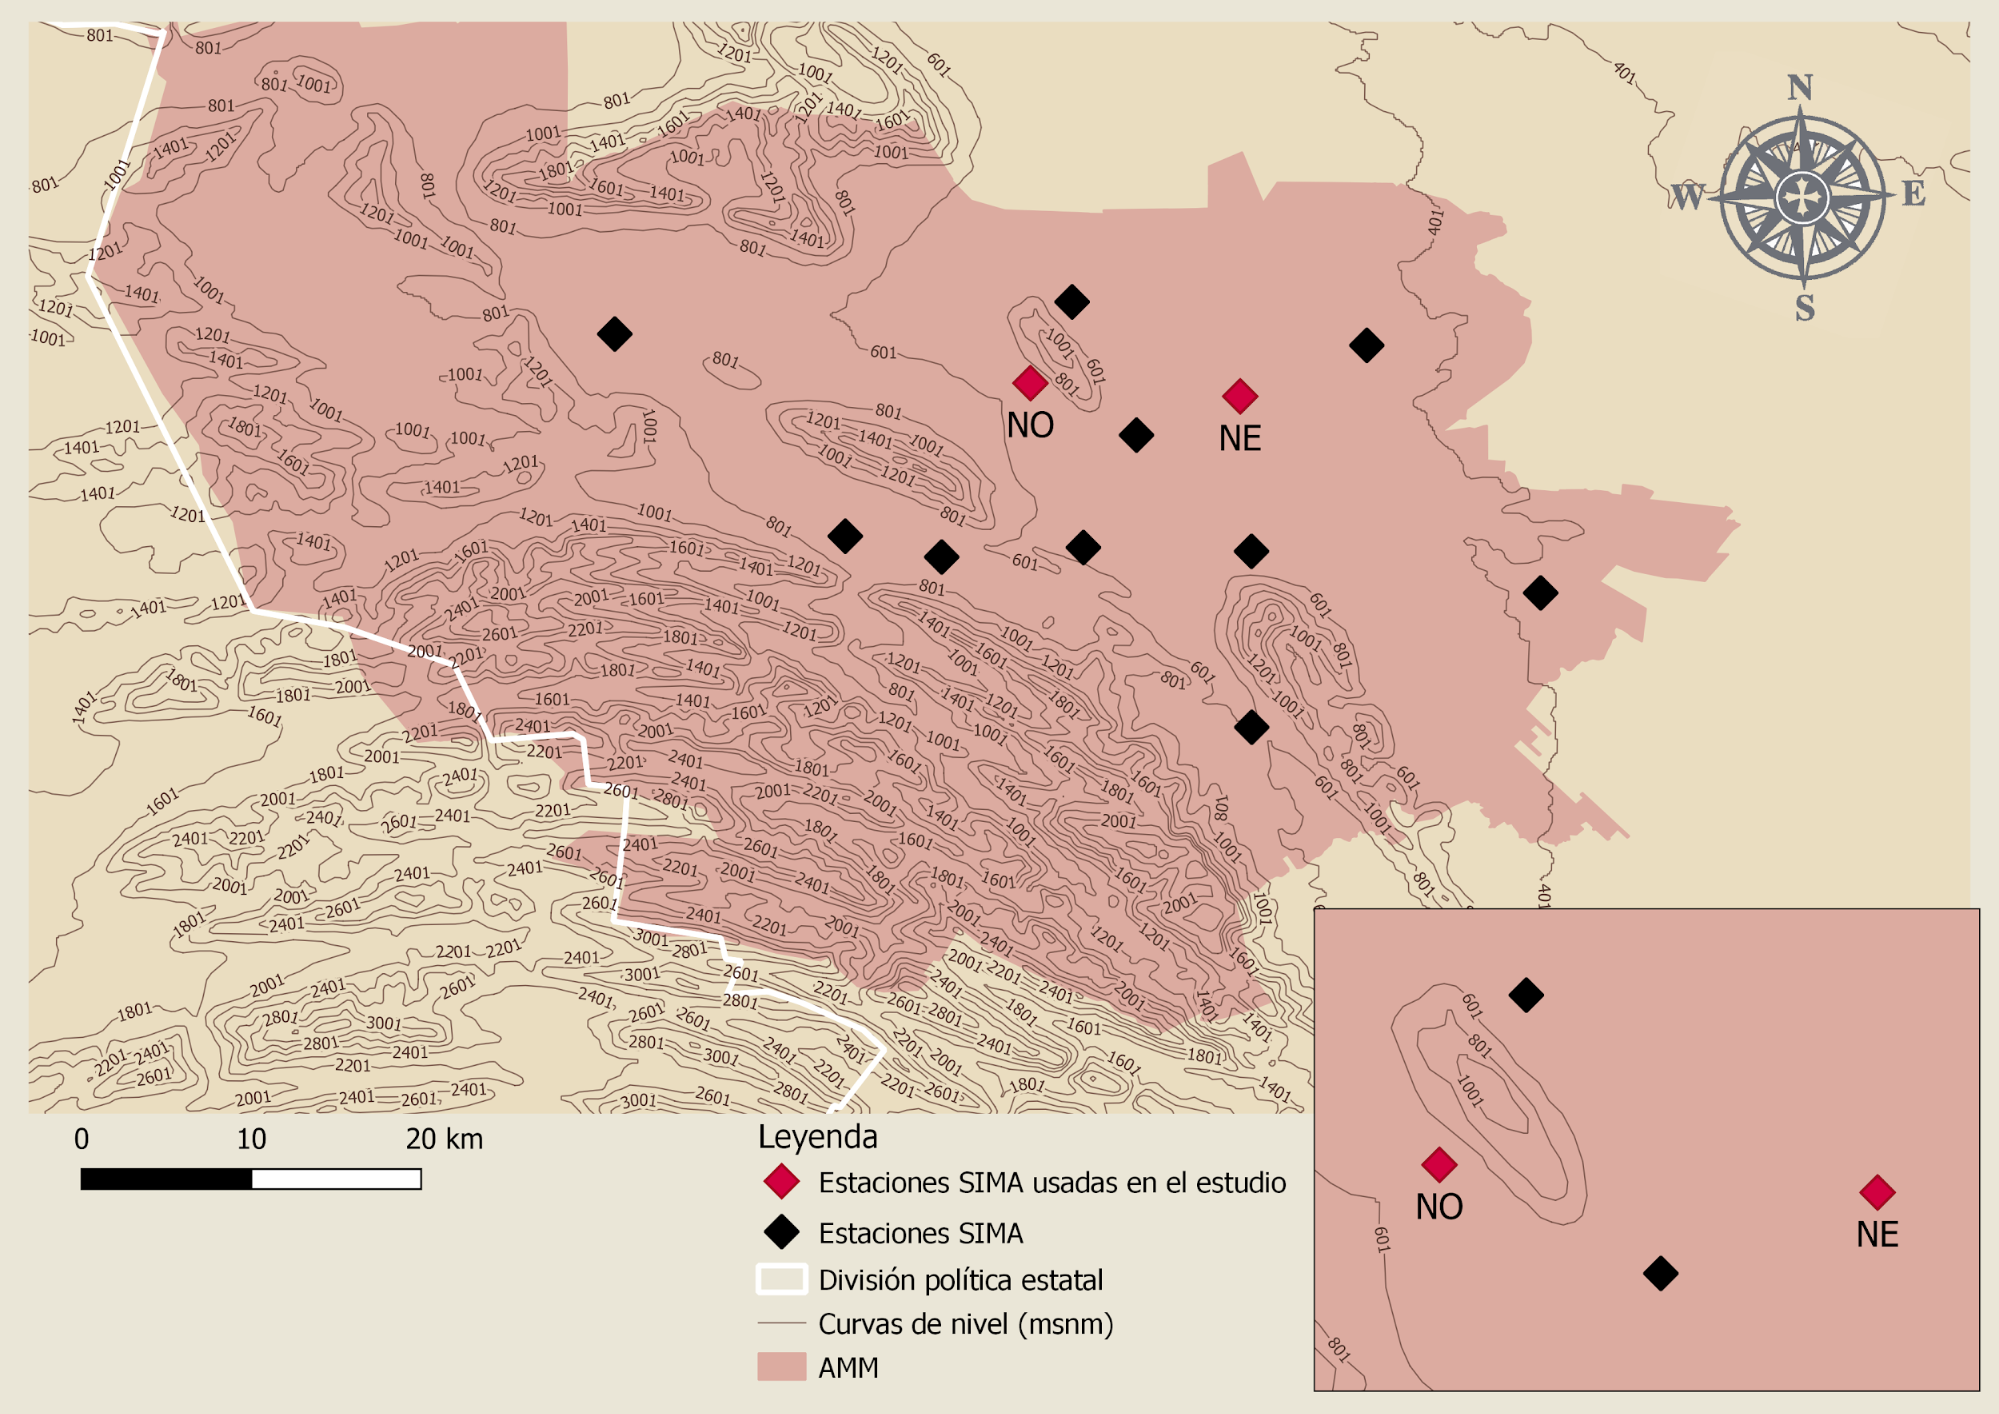
\includegraphics[scale=0.15]{images/map.png}
    \caption{Incluir locación de MMA en México (climas), distribución, estaciones y alturas}
    \label{fig:map}
\end{figure}
\subsection{Meteorology, solar irradiance and PM\textsubscript{10} measurements}
De las estaciones San Nicolas y San Bernabé se realizó un filtro de días de cielo despejado haciendo uso de las mediciones de irradiancia
solar en el rango 285nm a 2800nm. En la tabla \ref{table:measurements_SIMA} se muestra el porcentaje de mediciones anuales en cada estación de la red 
del SIMA, se relleno en rojo las estaciones que tienen un porcentaje menor a 75\%, ya que con esto se considera que
las mediciones no son representativas \cite{molina2019}.
\begin{table}[H]
    \changefontsizes{9pt}
    \begin{tabular}{lcccccccccccc}
        \hline
        \multicolumn{1}{c}{}                       & \multicolumn{2}{c}{2015} & \multicolumn{2}{c}{2016} & \multicolumn{2}{c}{2017} & \multicolumn{2}{c}{2018} & \multicolumn{2}{c}{2019}                            & \multicolumn{2}{c}{2020}                                                                                                                                                                                                    \\ \cline{2-13}
        \multicolumn{1}{c}{\multirow{-2}{*}{Code}} & PM\textsubscript{10}     & SR                       & PM\textsubscript{10}     & SR                       & PM\textsubscript{10}                                & SR                                                  & PM\textsubscript{10} & SR   & PM\textsubscript{10} & SR                                                  & PM\textsubscript{10}                                & SR   \\ \hline
        CE                                         & 94.6                     & 95.8                     & 97.0                     & 97.7                     & 96.8                                                & 98.2                                                & 94.8                 & 99.1 & 95.1                 & 94.5                                                & 92.8                                                & 96.5 \\
        N                                          & 76.8                     & 98.8                     & 98.1                     & 97.9                     & 93.0                                                & 96.6                                                & 94.1                 & 97.6 & 96.3                 & 99.9                                                & \cellcolor[HTML]{CB0000}{\color[HTML]{FFFFFF} 73.7} & 84.3 \\
        N2                                         & -                        & -                        & -                        & -                        & \cellcolor[HTML]{CB0000}{\color[HTML]{FFFFFF} 20.9} & \cellcolor[HTML]{CB0000}{\color[HTML]{FFFFFF} 25.1} & 94.3                 & 98.6 & 94.4                 & 98.8                                                & 92.3                                                & 99.1 \\
        NE                                         & 93.9                     & 83.9                     & 98.3                     & 96.9                     & 98.1                                                & 99.2                                                & 97.4                 & 99.8 & 98.5                 & 99.5                                                & 92.8                                                & 89.3 \\
        NE2                                        & 89.9                     & 98.3                     & 93.7                     & 99.9                     & 96.3                                                & 99.8                                                & 96.1                 & 99.4 & 94.5                 & 99.1                                                & 91.1                                                & 98.1 \\
        NW                                         & 95.3                     & 99.3                     & 98.1                     & 94.9                     & 98.5                                                & 99.7                                                & 94.9                 & 99.5 & 90.9                 & 94.4                                                & 96.5                                                & 98.7 \\
        NW2                                        & 83.8                     & 97.7                     & 84.3                     & 88.5                     & 95.7                                                & 99.0                                                & 96.6                 & 99.5 & 95.8                 & 98.2                                                & 96.4                                                & 99.4 \\
        S                                          & -                        & -                        & -                        & -                        & \cellcolor[HTML]{CB0000}{\color[HTML]{FFFFFF} 22.8} & \cellcolor[HTML]{CB0000}{\color[HTML]{FFFFFF} 23.7} & 92.9                 & 99.4 & 96.7                 & 99.6                                                & 94.8                                                & 99.9 \\
        SE                                         & 92.8                     & 98.6                     & 97.2                     & 99.0                     & 98.4                                                & 99.1                                                & 94.3                 & 98.5 & 95.9                 & 98.4                                                & 94.1                                                & 99.1 \\
        SE2                                        & 95.9                     & 99.6                     & 99.1                     & 100.0                    & 95.7                                                & 97.4                                                & 92.4                 & 99.6 & 95.8                 & \cellcolor[HTML]{CB0000}{\color[HTML]{FFFFFF} 64.2} & 90.3                                                & 99.7 \\
        SE3                                        & -                        & -                        & -                        & -                        & \cellcolor[HTML]{CB0000}{\color[HTML]{FFFFFF} 37.1} & \cellcolor[HTML]{CB0000}{\color[HTML]{FFFFFF} 38.6} & 95.1                 & 99.1 & 98.3                 & 99.8                                                & 94.1                                                & 99.7 \\
        SW                                         & 92.3                     & 97.2                     & 96.9                     & 98.7                     & 97.9                                                & 99.6                                                & 92.6                 & 99.2 & 97.9                 & 99.6                                                & 97.0                                                & 99.6 \\
        SW2                                        & 88.4                     & 96.5                     & 96.8                     & 98.6                     & 93.6                                                & 98.1                                                & 95.1                 & 99.5 & 96.7                 & 99.7                                                & 90.8                                                & 99.9 \\ \hline
    \end{tabular}
    \caption{Porcentaje anual de las mediciones de PM\textsubscript{10} e irradiancia solar de las estacion del SIMA en el periodo 2015-2020.}
    \label{table:measurements_SIMA}
\end{table}
Se seleccionaron las estaciones de San Nicolas y San Bernabé ya que estas contaban con una mayor cantidad de datos disponibles
y los radiómetros usados para las mediciones de irradiancia solar se sabían concretamente que miden en el rango 285-2800 nm.
Realizando una visualización de los datos, se seleccionaron los días de cielo despejado usando el criterio ()
como los que se muetran en la figura \ref{fig:clear_days}.
\begin{figure}[H]
    \centering
    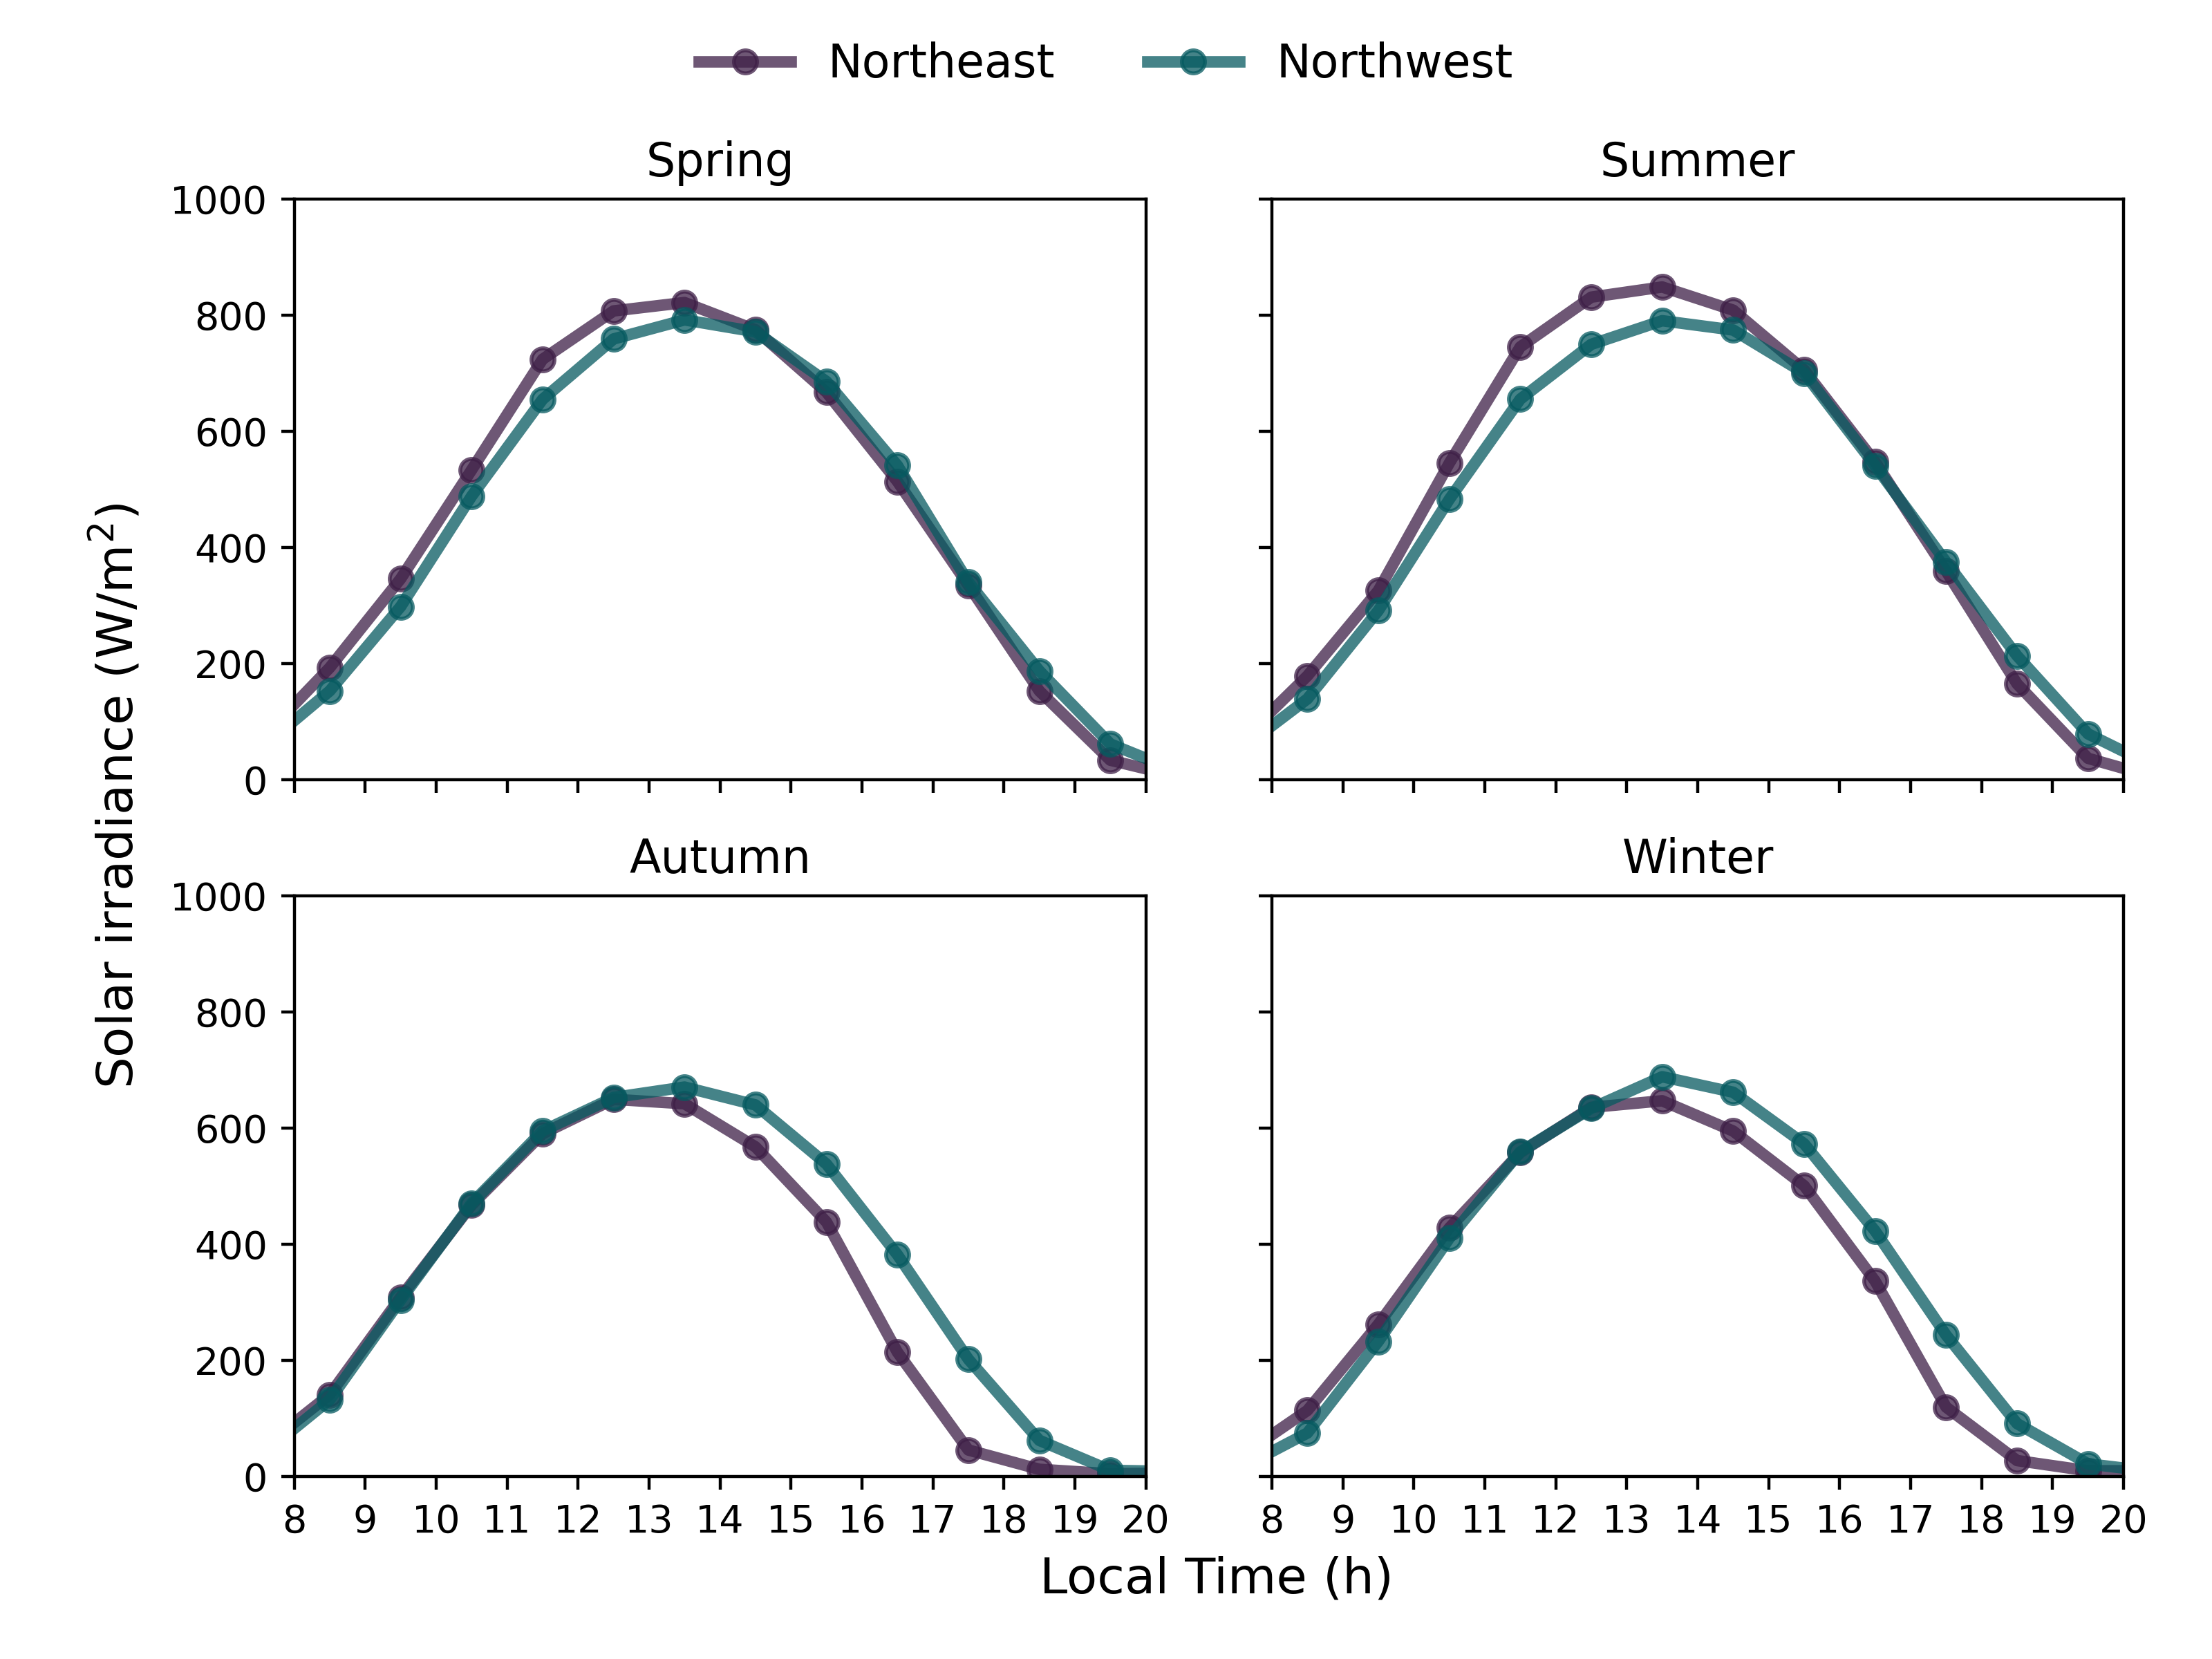
\includegraphics[scale=0.5]{images/Clear_days.png}
    \caption{}
    \label{fig:clear_days}
\end{figure}
\subsection{Satellite measurements}
\subsubsection{OMI-NASA Data}
Se utilizaron los datos de las columnas de Ozono (O\textsubscript{3}) en Dobson Units del satélite OMI de la NASA 
(\url{https://aura.gsfc.nasa.gov/omi.html}). Los datos fueron medidos diariamente con una resolución espacial de 0.25$^{\circ}$ Deg.
Tomamos el producto OMI/Aura Ozone DOAS Total Column L3 1 day V3 (OMDOAO3e), con un código escrito en \textit{Python} obtuvimos
los promedios mensuales para cada año para así dar un valor a los días en que no se tuvo una medición en la zona metropolitana de Monterrey.
\subsubsection{MODIS-NASA Data}
We download the data of Aerosol Optical Depth at 550 nm (AOD\textsubscript{550nm}) from NASA’s
satellite MODIS (\url{https://ladsweb.modaps.eosdis.nasa.gov/}). The data is taken daily and with a spatial
resolution of 1 Deg. We used the product MODIS-Aqua Aerosol Cloud Water Vapor Ozone Daily L3 Global 1Deg CMG
(MYD08\_D3) and looked at two data sets: Deep Blue Combined Mean and Land and Ocean Mean. 
\subsection{SMARTS Model}
El \textit{Simple Model of the Atmosphere Radiactive Transfer of Sunshine} (SMARTS) es un modelo de transferencia radiativa
escrito en el lenguaje \textit{Fortran}, el cual calcula la irradiancia solar directa, difusa y la 
global en cualquier ángulo en la superficie de la Tierra. Se creó un código en
\textit{Python} que realizá la lectura de los parámetros de la tabla \ref{table:parameters} y escribe los datos de entrada 
en el formato del modelo SMARTS. 
\begin{table}[H]
    \centering
    \begin{tabular}{lcccc}
        \hline
        \multicolumn{1}{c}{\multirow{2}{*}{Parameters}} & \multicolumn{4}{c}{Stage}                                          \\ \cline{2-5}
        \multicolumn{1}{c}{}                            & Pristine                  & Moderate & SSA Pristine & SSA Moderate \\ \hline
        $\alpha_1$                                      & 0.8565                    & 0.8565   & 1.0          & 1.0          \\
        $\alpha_2$                                      & 1.2037                    & 1.2037   & 1.0          & 1.0          \\
        SSA\textsubscript{500}                          & 0.6536                    & 0.6536   & 0.8          & 0.8          \\
        g\textsubscript{500}                            & 0.6783                    & 0.6783   & 0.68         & 0.68         \\
        CH\textsubscript{2}O                            & -0.003                    & 0.007    & -0.003       & 0.007        \\
        CH\textsubscript{4}                             & 0                         & 0.3      & 0            & 0.3          \\
        CO                                              & -0.1                      & 0.35     & -0.1         & 0.35         \\
        HNO\textsubscript{3}                            & 0                         & 0.005    & 0            & 0.005        \\
        NO                                              & 0                         & 0.2      & 0            & 0.2          \\
        NO\textsubscript{2}                             & 0                         & 0.02     & 0            & 0.02         \\
        O\textsubscript{3}                              & -0.007                    & 0.053    & -0.007       & 0.053        \\
        SO\textsubscript{2}                             & 0                         & 0.05     & 0            & 0.05         \\ \hline
    \end{tabular}
    \caption{$\alpha_1$: \AA ngstr\"om for $\lambda<500$nm,
        $\alpha_2$: \AA ngstr\"om  for $\lambda>500$nm,
        SSA$_{500}$: Single scatterging Albedo at 500nm,
        g$_{500}$: Asymmetry factor ait 500nm.}
    \label{table:parameters}
\end{table}
\subsubsection{Algortimo para determinar el AOD correspondiente a la medición}
A partir de la selección de los días de cielo despejado se creó una base de datos que contiene:
día, mes y año en formato yymmdd, columna total de ozono (TOC) OMI-NASA, con las coordenadas geográficas
para cada estación de monitoreo, pueden tener días de cielo despejado diferentes.
Se escribió un código en el lenguaje \textit{Python}, el cual creará el archivo de input para el modelo SMARTS usando
un AOD inicial de 0.5. El modelo SMARTS da como resultado una matriz de espectros solares por cada  minuto entre las 9 y 16 horas,
el código de python calcula la irradiancia solar con base a la ecuación \ref{eq:irradiance}.
\begin{equation}
        I(t) = \int\limits_{285}^{2800} E(\lambda,t) d\lambda
        \label{eq:irradiance}
\end{equation}
Al tener la irradiancia solar diaria, se establece el valor máximo de irradiancia solar y se calcula el promedio 
centrado en 1 hora. Se obtiene la diferencia relativa entre el promedio de la irradiancia solar máxima medida y
la obtenida con el modelo por medio de la ecuación \ref{eq:rd}. Dependiendo de que valor tenga la diferencia relativa
se asignará un valor al AOD, este procedimiento realiza el siguiente algortimo:
\begin{enumerate}
    \item Si la diferencia relativa tiene un valor mayor a 11\%, entonces el límite inferior es el AOD con el cual se produjo esa diferencia relativa, al inicio del proceso el límite inferior del AOD es 0.01.
    \item Si la diferencia relativa tiene un valor menor a 9\%, entonces el límite superior es el AOD con el cual se produjo esa diferencia relativa, al inicio del proceso el límite superior del AOD es 1.
    \item En cualquiera de los dos casos, el nuevo valor del AOD es un promedio del límite inferior y superior.
    \item Este proceso termina cuando se obtiene una diferencia relativa entre 9\% y 11\% o el número de intentos es 10. Si la diferencia relativa se encuentra entre 9\% y 11\% este valor es guardado en una base de datos.
\end{enumerate}
\begin{equation}
    RD = \left(\frac{Model-Measurement}{Measurement}\right)*100\%
    \label{eq:rd}
\end{equation}